% Section content template for individual Educative lessons
% This file contains the actual content for a specific section
% Generated from Educative API section content

% Section: Class Diagram for the Jigsaw Puzzle
% Section ID: 4983682953904128
% Section Slug: class-diagram-for-the-jigsaw-puzzle
% Generated: 2025-12-14T13:10:54.520338

In this lesson, we'll identify and design the classes, abstract classes, and interfaces based on the requirements we previously gathered from the interviewer in our jigsaw puzzle.

\subsection{Components of a jigsaw puzzle}\label{SvY19tM7F-lGSssRJvgGm}
\\
As mentioned, we should design the jigsaw puzzle using a bottom-up approach.

\subsubsection{Side}\label{DPTzRoMZDlx8e_jvZBIOR}
\\
The \texttt{Side} class represents the shape of our jigsaw piece and whether it contains an indentation, extrusion, or flat edge. The UML representation of the class is shown below:

\begin{figure}[htbp]
 \centering
 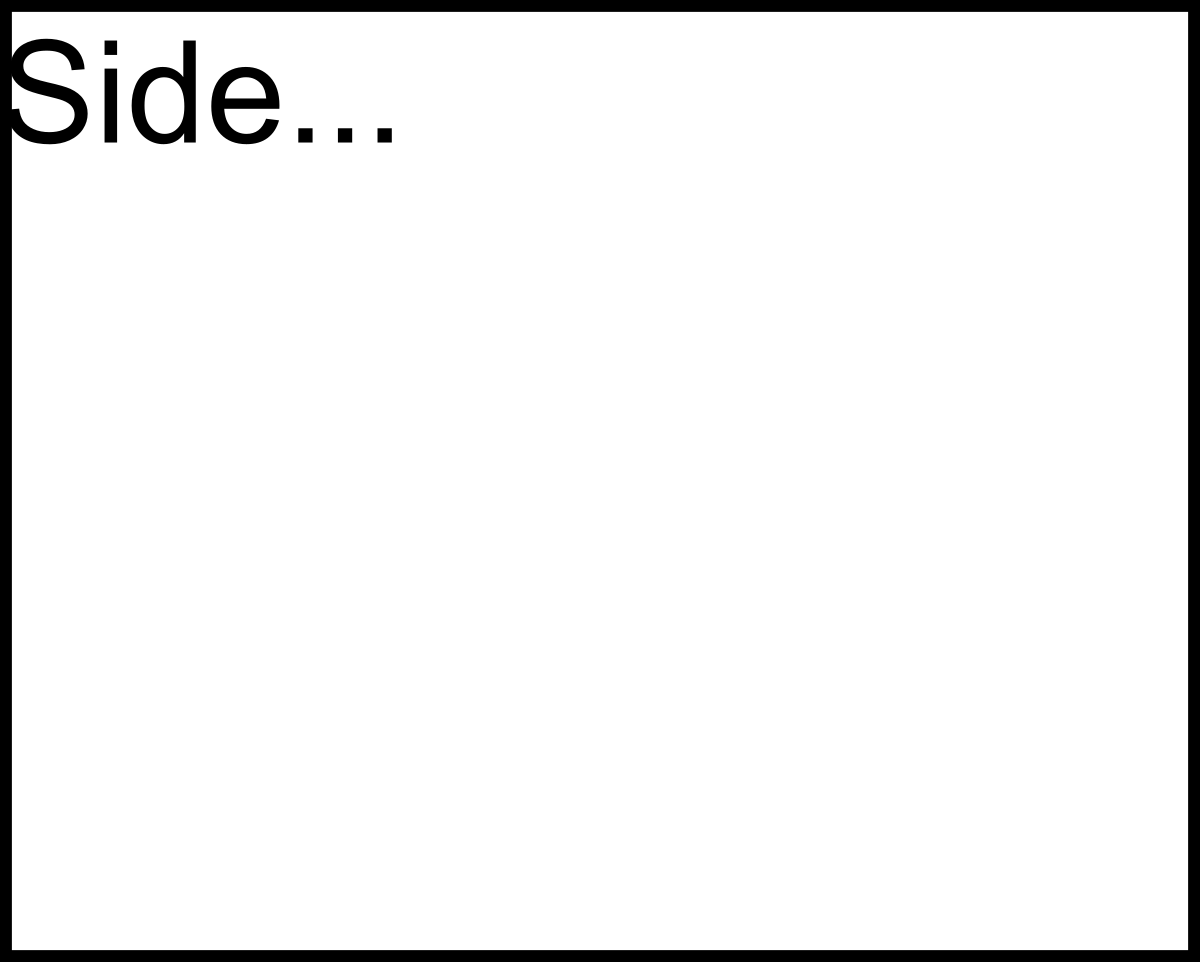
\includegraphics[width=0.5\textwidth]{Images/chapter_24/section_4983682953904128/4799460699013120.png}
 \caption{The class diagram of the Side class}
\end{figure}

\textbf{R2:} All pieces will have four sides with an indentation, an extrusion, or a flat edge.

\subsubsection{Piece}\label{givU1i2ycz7jmqXLVPTx8-1}
\\
The \texttt{Piece} class contains an array of sides of size four. It will also identify middle, corner, and edge pieces. The class representation of the \texttt{Piece} class is provided below:

\begin{figure}[htbp]
 \centering
 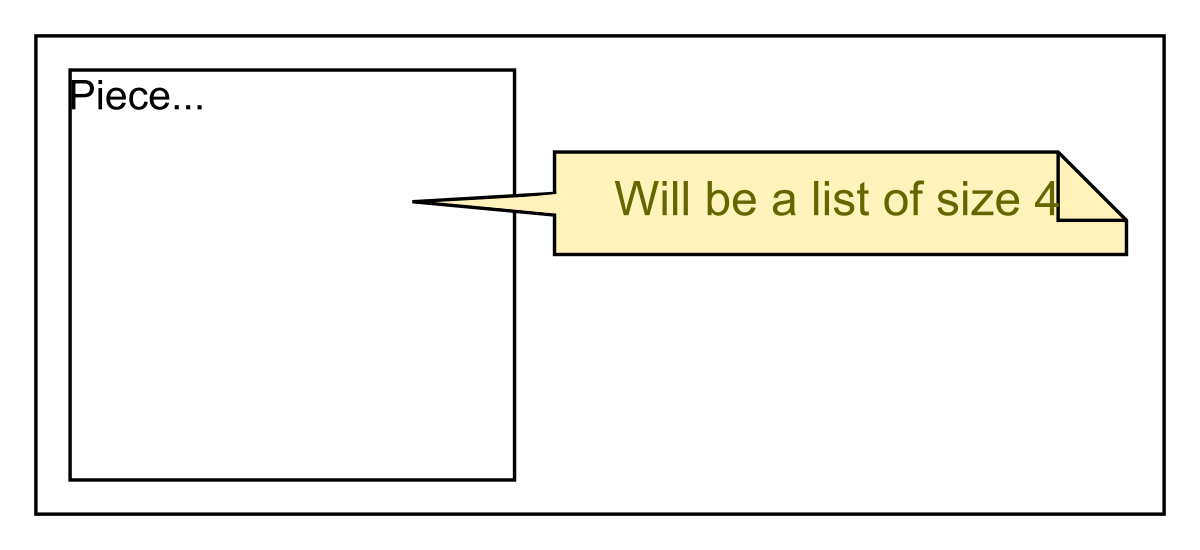
\includegraphics[width=0.5\textwidth]{Images/chapter_24/section_4983682953904128/5576647448068096.png}
 \caption{The class diagram of the Piece class}
\end{figure}

\textbf{R2:} All pieces will have four sides with an indentation, an extrusion, or a flat edge.
\\
\textbf{R3:} There are four corner pieces, some edge pieces, and the remaining ones are middle pieces. A corner piece has two flat sides, an edge piece only has one flat side, and a middle piece has no flat edges.

\subsubsection{Puzzle}\label{n3AHKWJcxUbAtZ0q9tOSG}
\\
The \texttt{Puzzle} class represents the board of our jigsaw game. As our board is a rectangle, it will be represented by a 2D array. There will also be a 1D array to represent the unused free pieces yet to be inserted into the puzzle board. It will also have the \texttt{insertPiece()} function to insert the piece into the board, ensuring that it is unique from its counterparts and only in the specified row and column.
\begin{quote}
\textbf{Note:} The puzzle board does not yet have the functionality of rotating pieces, so all pieces must be unique to fit into the board and solve the puzzle.
\end{quote}
\\
This class is represented below:

\begin{figure}[htbp]
 \centering
 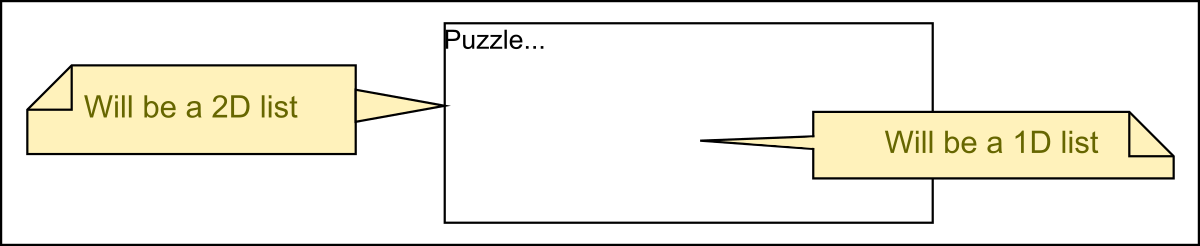
\includegraphics[width=0.5\textwidth]{Images/chapter_24/section_4983682953904128/5066173009231872.png}
 \caption{The class diagram of the Puzzle class}
\end{figure}

\textbf{R1:} Our board will be shaped like a rectangle.
\\
\textbf{R4:} All pieces will be unique, so only one piece will fit with only one other piece.

\subsubsection{Puzzle solver}\label{givU1i2ycz7jmqXLVPTx8-2}
\\
The \texttt{PuzzleSolver} class is responsible for solving an unsolved jigsaw puzzle board using its \texttt{matchPieces()} function. The visual representation of this class is given below:

\begin{figure}[htbp]
 \centering
 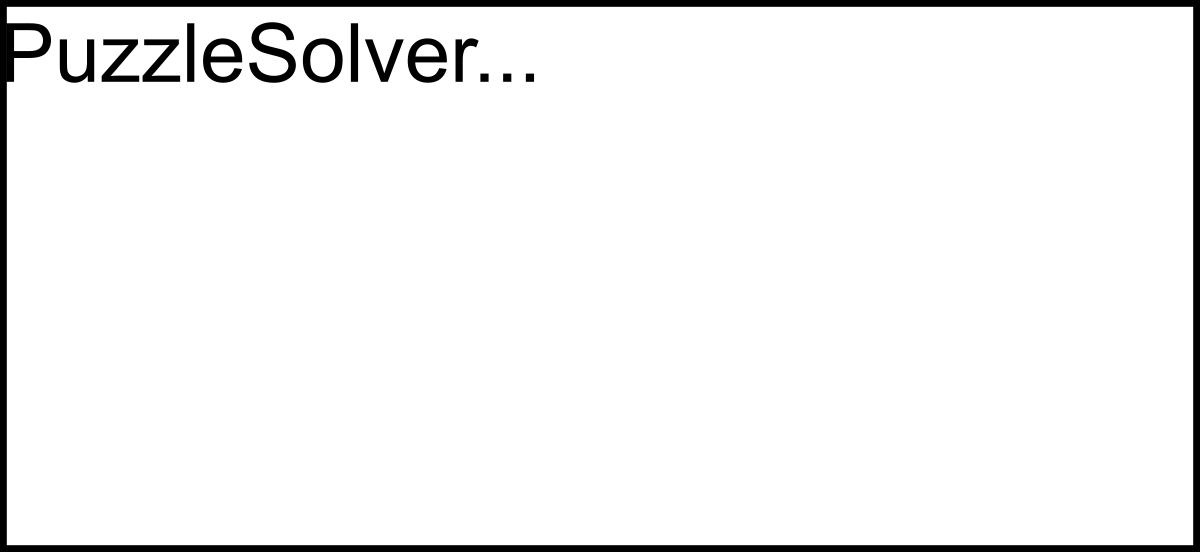
\includegraphics[width=0.5\textwidth]{Images/chapter_24/section_4983682953904128/6316322407579648.png}
 \caption{The class diagram of the PuzzleSolver class}
\end{figure}

\textbf{R5:} Two pieces fit together by the curvature of the indentation on one piece matching up to the curvature of the extrusion on another.

\subsubsection{Edge enumeration}\label{spPUwOm3kRzPiqkKehu98}
\\
The \texttt{Edge} enum describes the various edges present in a jigsaw puzzle piece. It is represented using the class diagram given below:

\begin{figure}[htbp]
 \centering
 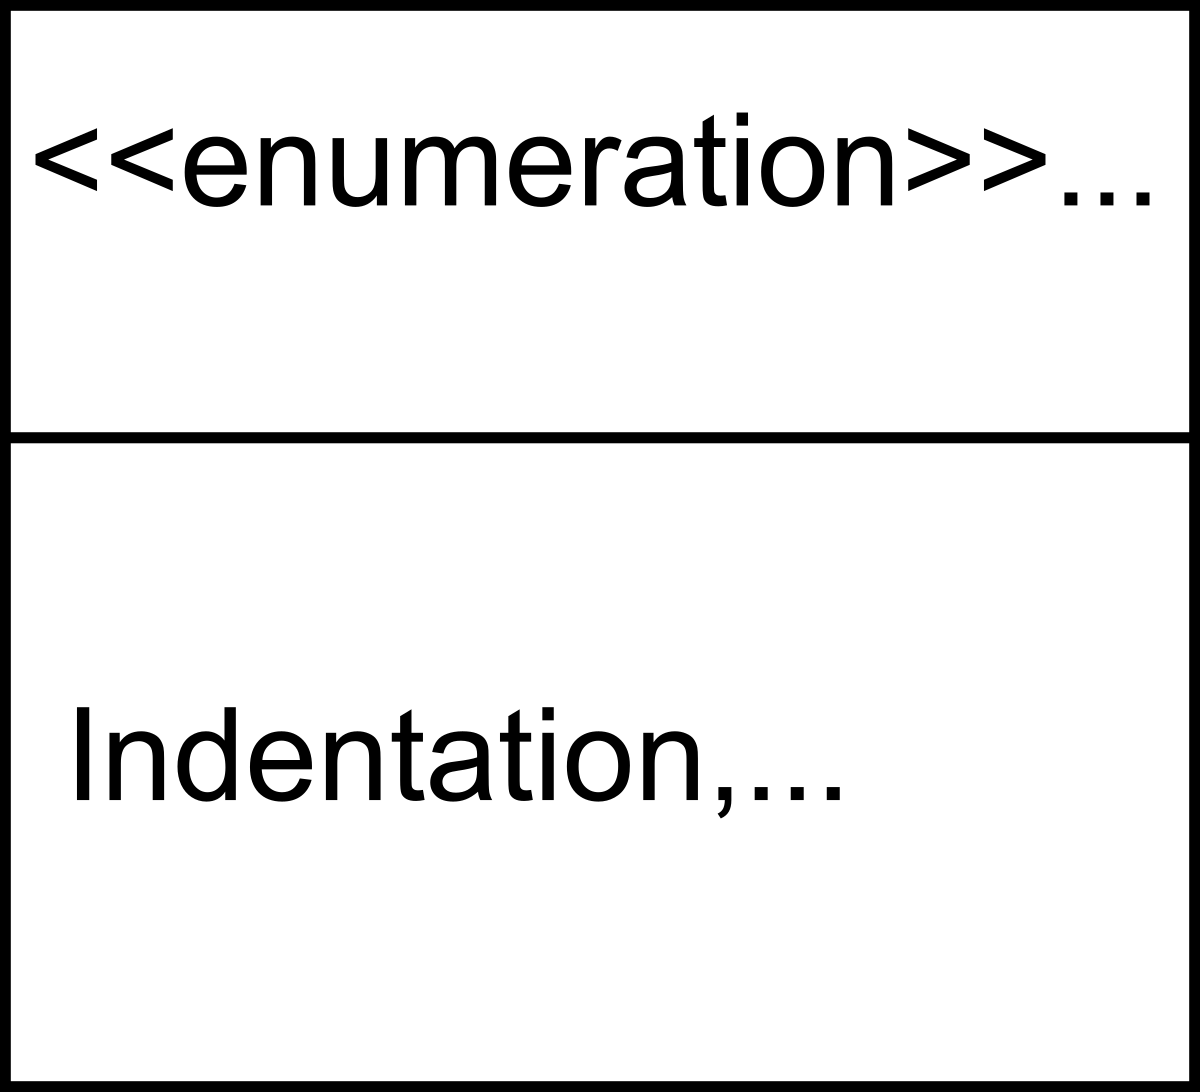
\includegraphics[width=0.5\textwidth]{Images/chapter_24/section_4983682953904128/5394761604399104.png}
 \caption{The class diagram of the Edge enum}
\end{figure}

\subsection{Relationship between the classes}\label{givU1i2ycz7jmqXLVPTx8-3}
\\
Now, we'll discuss the relationships between the classes we have defined above in our jigsaw puzzle.

\subsubsection{Association}\label{uVXxAi-lfaqirKwQj0zxJ}
\\
The class diagram has the following association relationships:

\begin{itemize}
\item
\protect\phantomsection\label{vyDk9FOdrDo3hcNzVEu1e}
The \texttt{Puzzle} has a one-way association with \texttt{PuzzleSolver}.
\end{itemize}

\begin{figure}[htbp]
 \centering
 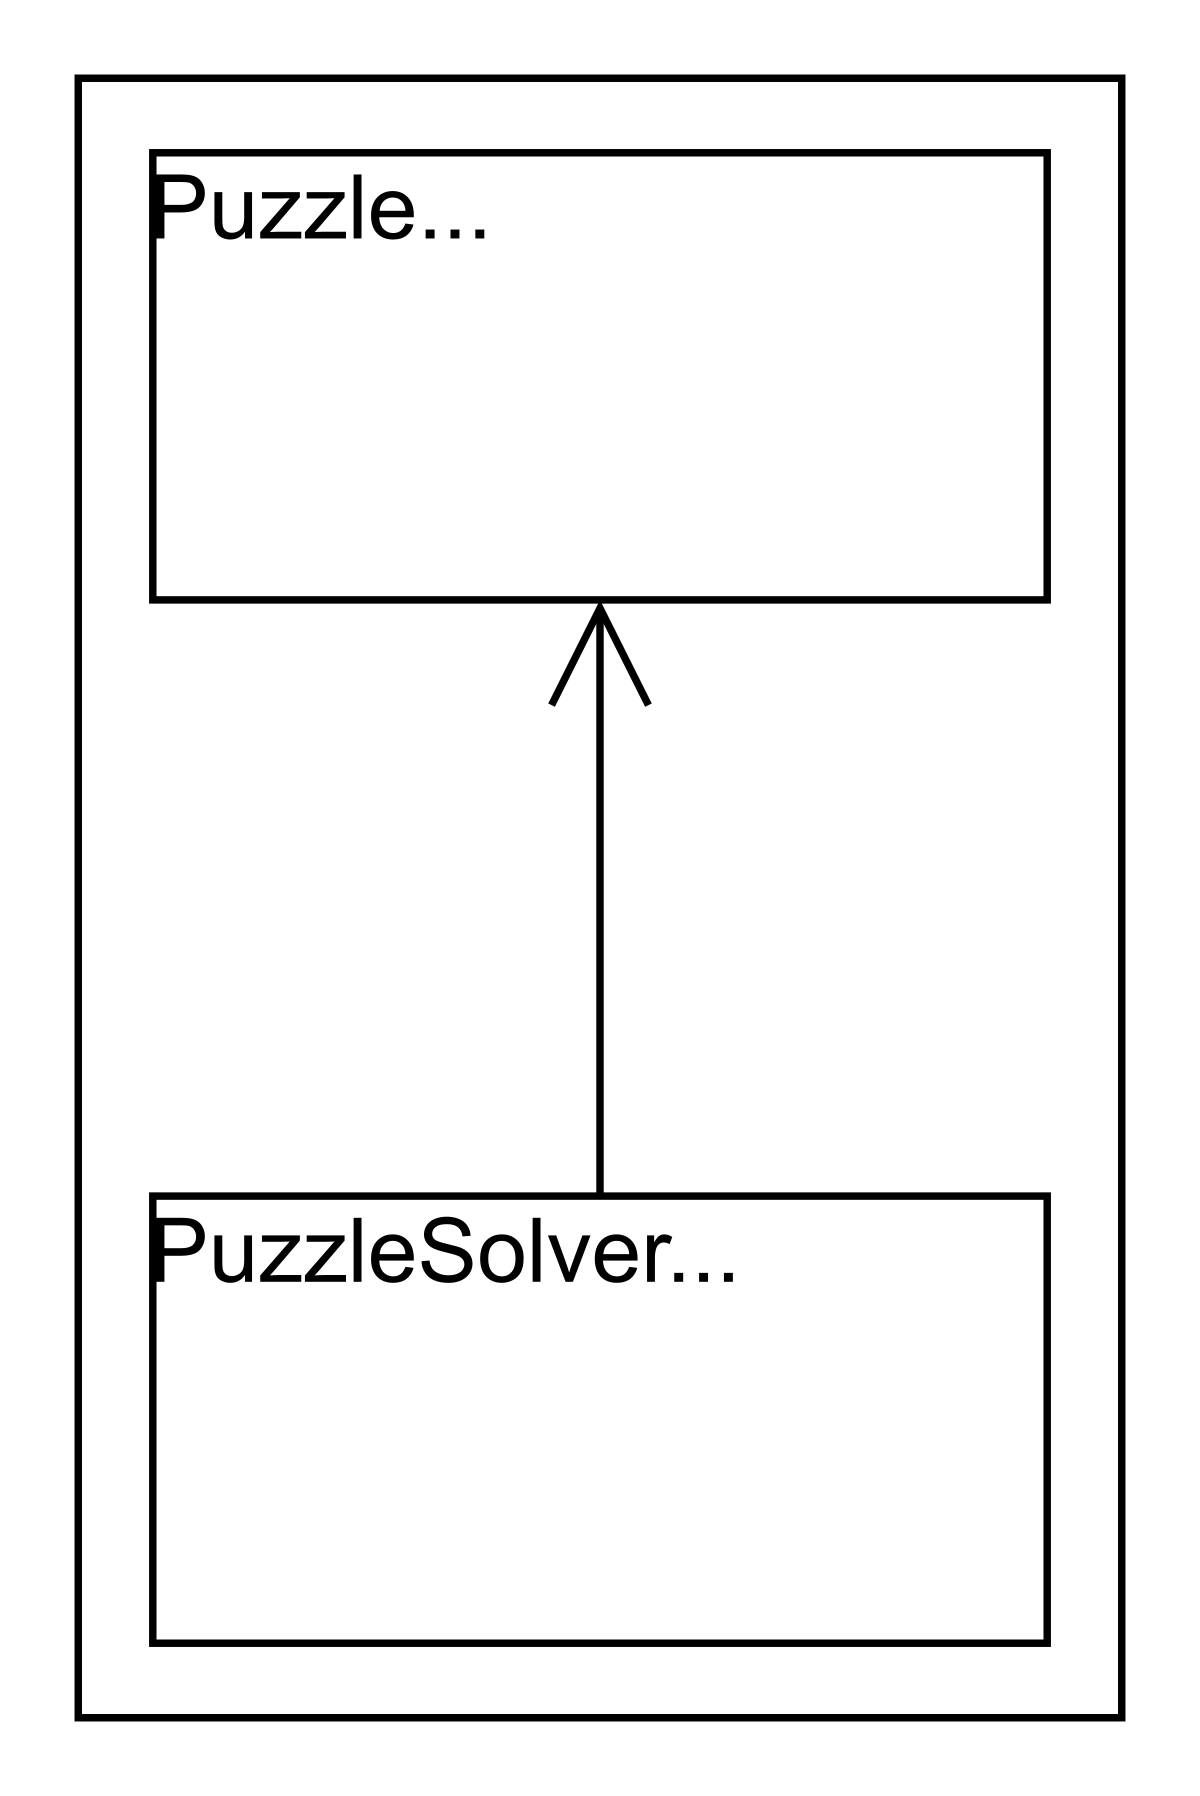
\includegraphics[width=0.5\textwidth]{Images/chapter_24/section_4983682953904128/6059171387408384.png}
 \caption{The association relationship between classes}
\end{figure}

\subsubsection{Composition}\label{givU1i2ycz7jmqXLVPTx8-4}
\\
The class diagram has the following composition relationships:

\begin{itemize}
\item
\protect\phantomsection\label{wcL4Bm9hRDZ-N9bDeQPE0}
The \texttt{Puzzle} class is composed of the \texttt{Piece} class, which is composed of the \texttt{Side} class.
\end{itemize}

\begin{figure}[htbp]
 \centering
 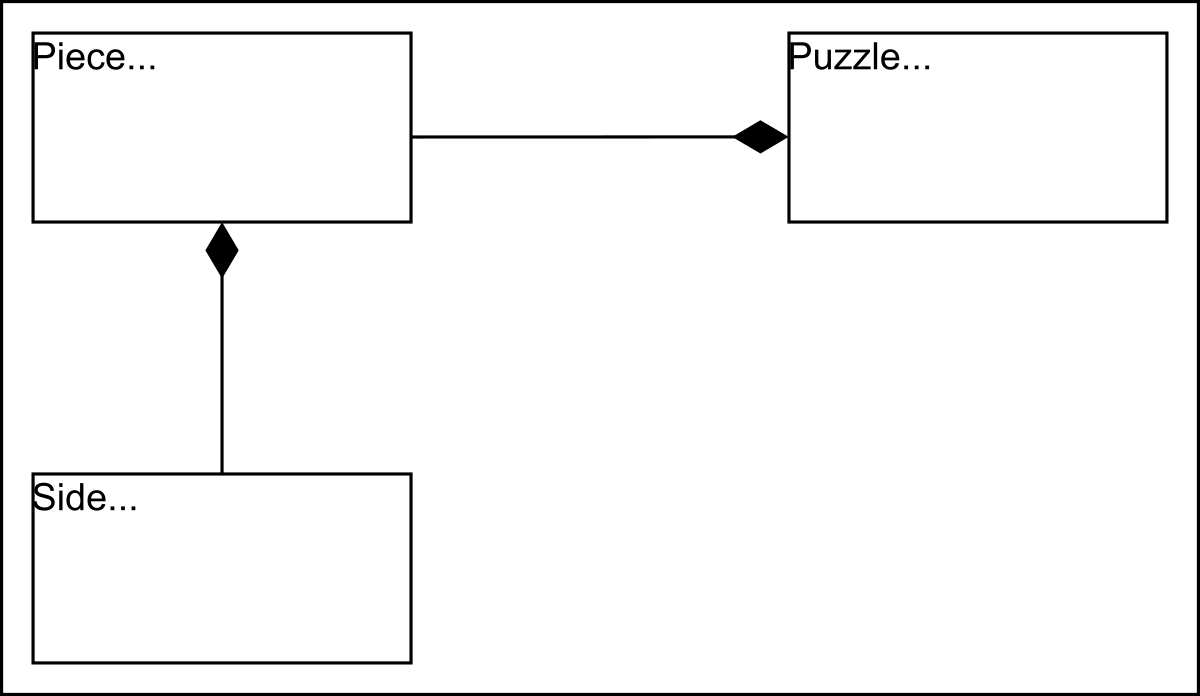
\includegraphics[width=0.5\textwidth]{Images/chapter_24/section_4983682953904128/5685220662837248.png}
 \caption{The composition relationship between classes}
\end{figure}

\subsection{Class diagram for the jigsaw puzzle}\label{givU1i2ycz7jmqXLVPTx8-5}
\\
Here's the complete class diagram for our jigsaw puzzle:

\begin{figure}[htbp]
 \centering
 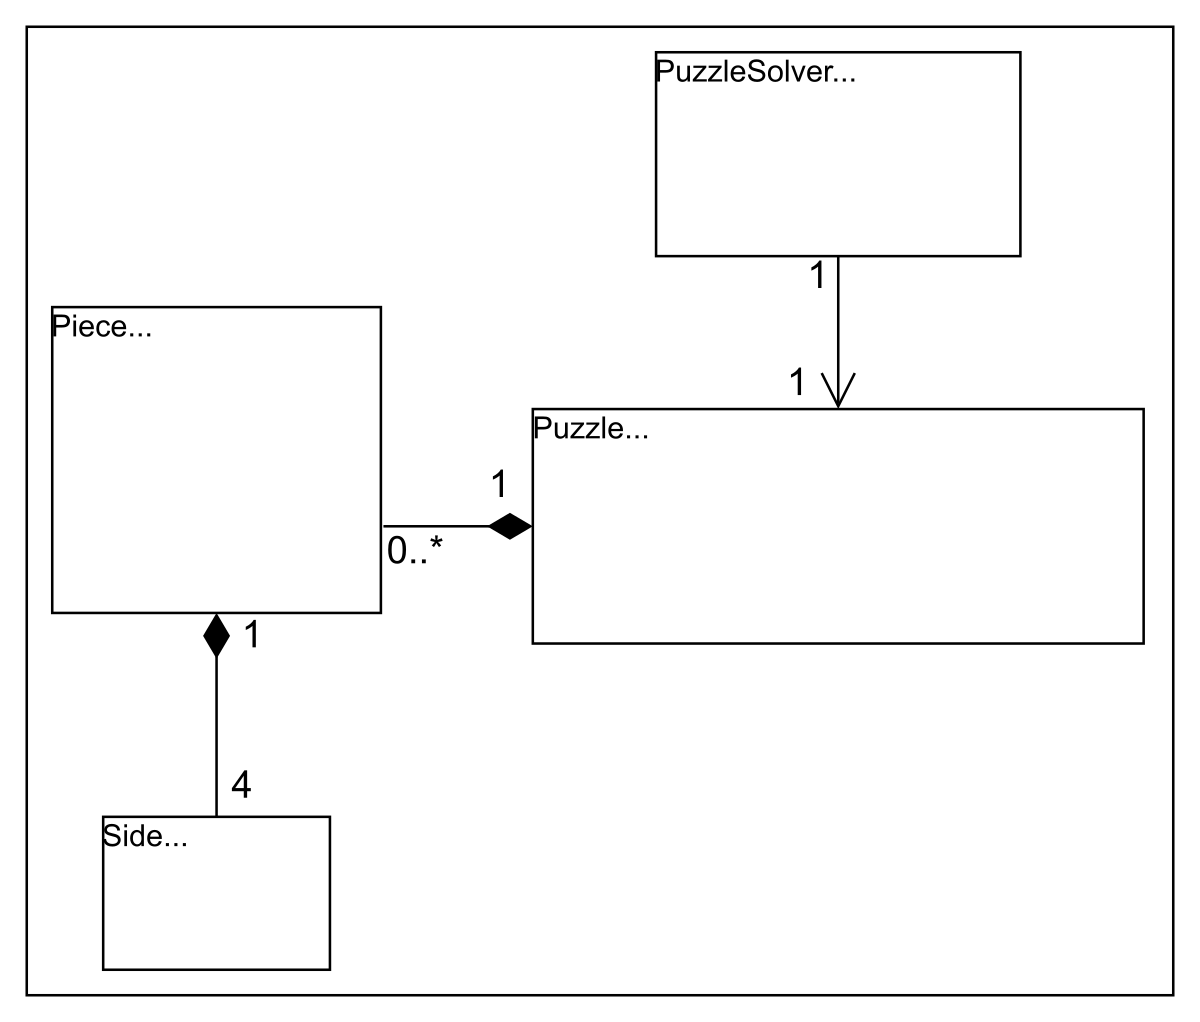
\includegraphics[width=0.5\textwidth]{Images/chapter_24/section_4983682953904128/6275823295135744.png}
 \caption{The class diagram of the jigsaw puzzle}
\end{figure}

\subsection{Design pattern}\label{6Qpgp8tFIWMNl81WuGthE}
\\
The jigsaw puzzle has only one instance of the puzzle board. Therefore, we use the Singleton design pattern to ensure that only one instance of the board is created using a special creation method, and this instance has a global point of access.

\subsection{AI-powered trainer}\label{Mtmnhz-DrwFdTSoz6z5HY}
\\
At this stage, everything should be clear. If you encounter any confusion or ambiguity, feel free to utilize the interactive AI-enabled widget below to seek clarification. This tool is designed to help you strengthen your understanding of the concepts.

\begin{figure}[htbp]
 \centering
 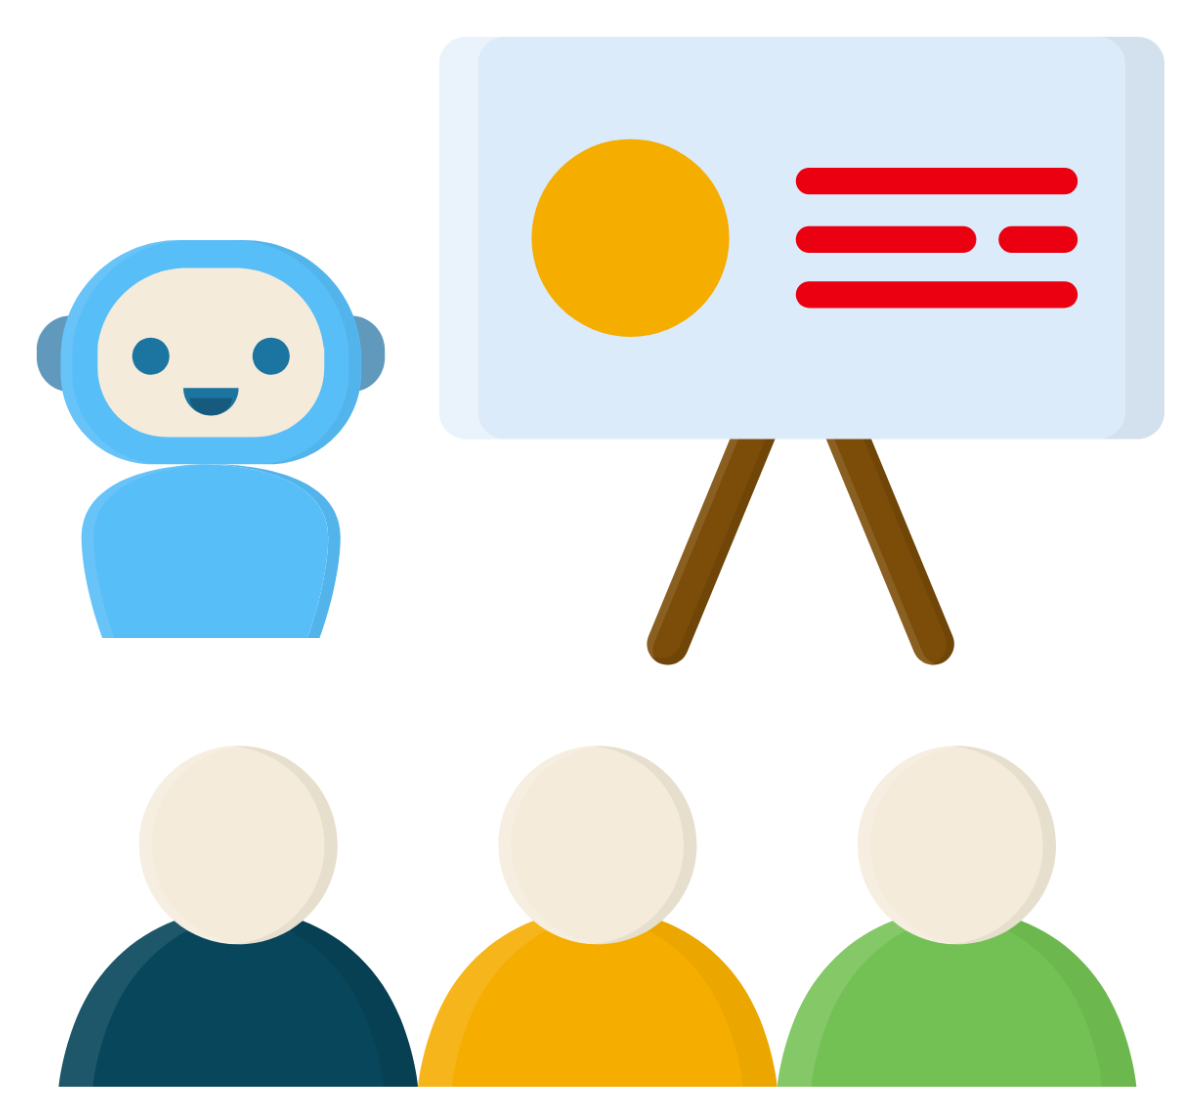
\includegraphics[width=0.15\textwidth]{Images/chapter_24/section_4983682953904128/5676853451685888.png}
 
\end{figure}

\subsection{Additional requirements}\label{5Qk5vSCn53GK0TfHAqj0N}
\\
The interviewer can introduce some additional requirements in the jigsaw puzzle, or they can ask some follow-up questions. ~Let's see some examples of additional requirements:
\\
\textbf{Rotate piece:} Pieces can be rotated to fit on the puzzle. The class diagram provided below shows the added functionality of rotation in the \texttt{Piece} class:

\begin{figure}[htbp]
 \centering
 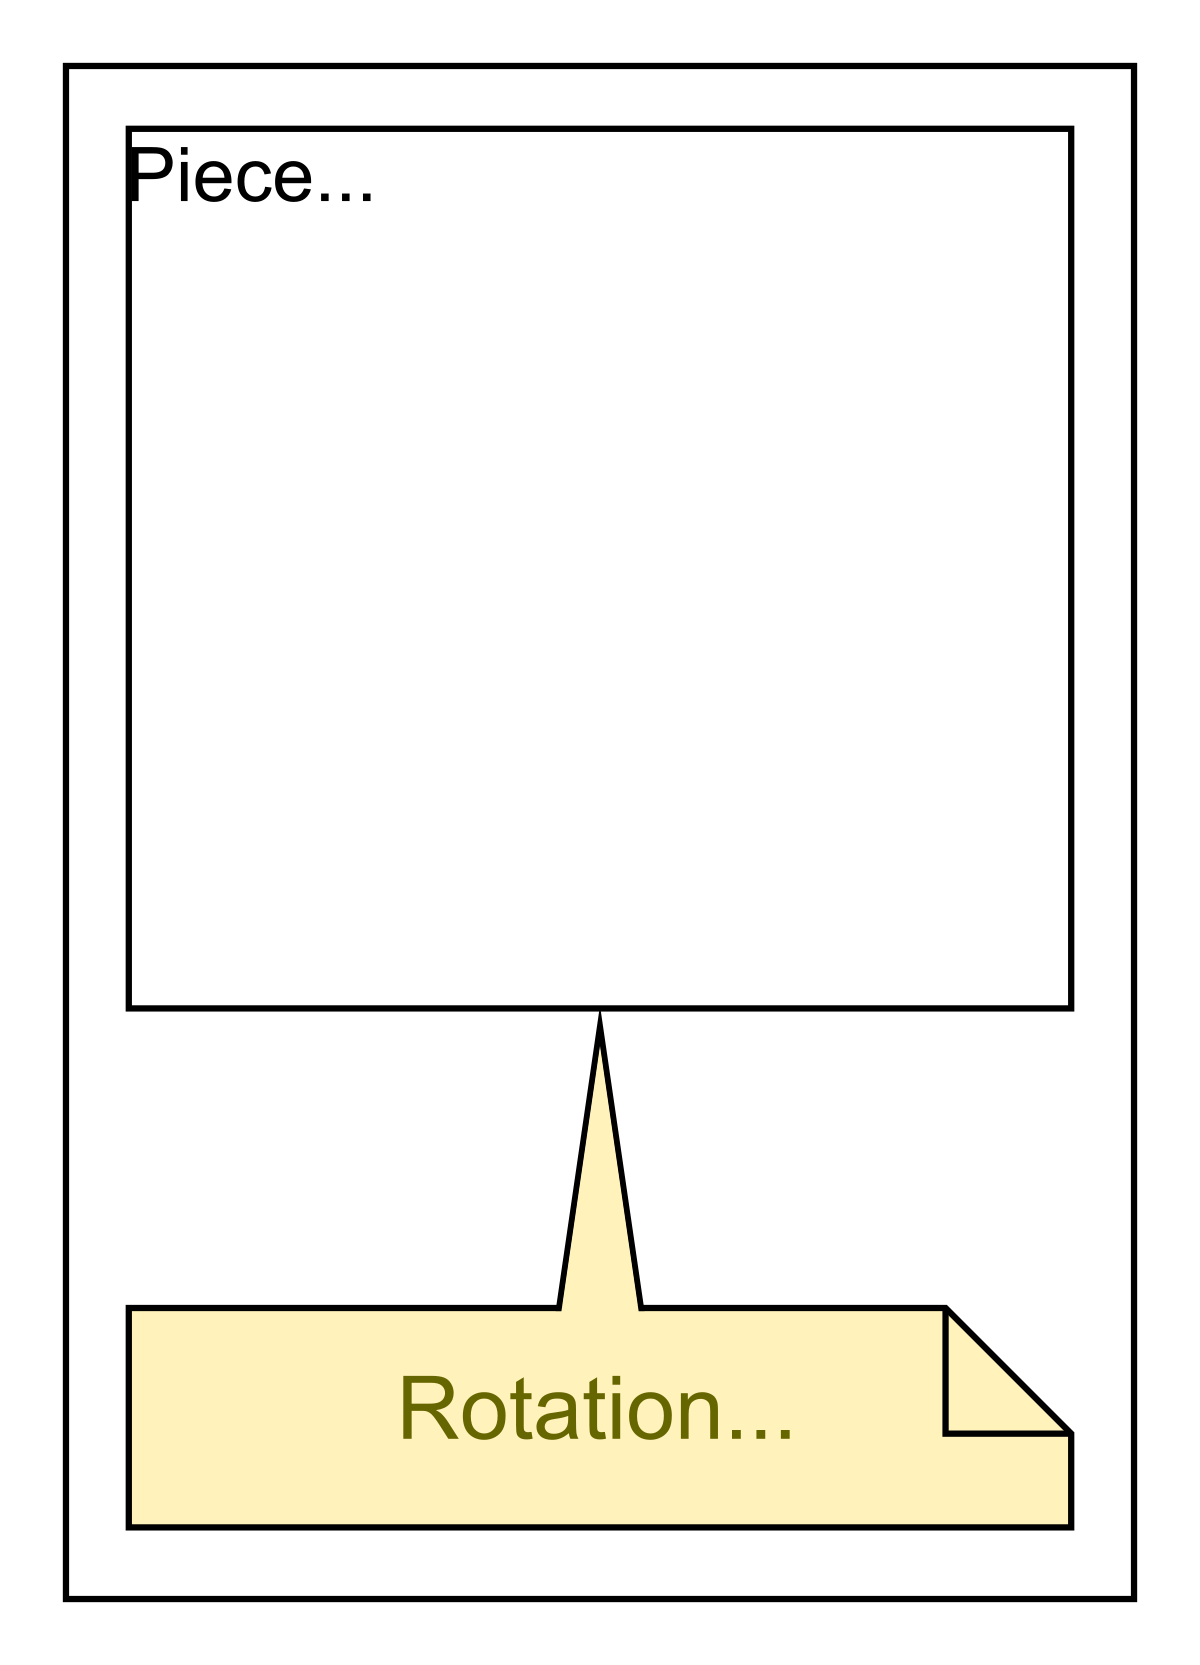
\includegraphics[width=0.5\textwidth]{Images/chapter_24/section_4983682953904128/5199220989362176.png}
 \caption{The class diagram of the rotation functionality in the Piece class}
\end{figure}

We have completed the class diagram of the jigsaw puzzle according to the requirements. ~Let's write the code for our designed classes in some popular languages.

% End of section content